\documentclass[fontsize=11pt]{article}
\usepackage{amsmath}
\usepackage{graphicx}
\usepackage[utf8]{inputenc}
\usepackage[margin=0.75in]{geometry}

\title{CSC110 Project Proposal:An Investigation of the Impact of COVID-19 on the  Political Satisfaction of the General Public}
\author{Aviraj Newatia, Mishaal Kandapath, Rudraksh Monga, Taylor Whatley}
\date{Friday, November 5, 2021}

\begin{document}
\maketitle

\section*{Problem Description and Research Question}

Politics is a very polarizing field of study - even before COVID-19, political opinions varied vastly among differing political ideologies, but ever since the coronavirus went viral the onset of political mistrust, misinformation, and fake news has made the political landscape even more difficult to navigate. The public political opinion in countries such as Bosnia and Herzegovina, for example, was largely negative as many blamed the government for prematurely opening the border, leading to increased death rates, while the public’s political opinion in other countries such as China, for example, was largely positive due to the efficacy with which it handled the pandemic [1]. Considering how many countries were affected by COVID-19, our group decided to narrow our focus to just one country, the US, because of its economic importance in the global economy and because of how much the country has stood out during the pandemic (due to things such as Donald Trump’s infamous “disinfectant” cure). Given how governmental decisions could cost the lives of hundreds during the pandemic, our group decided that it would be best for us to analyse the US public’s opinions with the government during this pandemic. 
\\\\
Reddit [https://www.reddit.com/] is a social media website revolving around user-led communities. It has been typically perceived as a digital platform for people to express their opinions, especially for younger populations with access to the Internet. Subreddits such as r/usapolitics have been integral platforms for the community’s expression of their political opinions, especially during periods of political unrest or public disapproval (such as during elections or pandemics). Being active members of the Reddit community ourselves, our group decided to look at how people’s political opinions, as expressed on various different subreddits, changed during the progression of COVID-19 because we believe that people tend to be more honest on online forums where they can remain anonymous [2]. Additionally, our group wanted to know whether key moments during the pandemic led to drastic changes in people’s political opinions or not. As such, to find answers to our questions our group has decided to answer the question of \textbf{“How Has the Political Satisfaction of the General Public Changed During the COVID-19 Pandemic?”}

\section*{Dataset Description}

The dataset we will be using was sourced from the online machine learning data repository Kaggle, a subsidiary of Google LLC, which serves as an online community of data scientists and machine learning practitioners.
\\\\
It is a csv (comma-separated values) file of 17,777,472 unique comments related to covid that were collated from the online forum platform Reddit. The dataset is called The Reddit COVID dataset [https://www.kaggle.com/pavellexyr/the-reddit-covid-dataset].
\\\\
We transformed this dataset by filtering by the subreddit the comment came from, building a sub-dataset of comments only from political subreddits such as r/uspolitics.
\\\\
The dataset was too large to load into Excel, so we filtered our dataset to include only U.S-related comments using Pandas in Python to yield 2295 comments.
\\\\
The dataset has 10 columns, of which we extracted and will be using 2 which are the actual text of the comment ("body") and the timestamp of creation/posting ("created\_utc"). \\\\
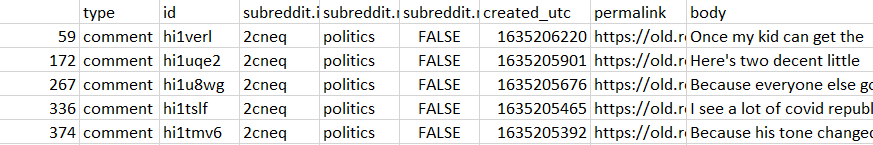
\includegraphics{rows.png}

\section*{Computational Plan}

Since the data is in a csv file, we intend to use the Pandas module due to its incredible utility and efficiency in handling large csv datasets. We plan on using the loc, iloc, to\_numpy, groupby methods for more selective access to and analysis on specific subsets in our dataset.
\\\\
Since our study is limited to U.S politics, we will be filtering out the dataset for subreddits related to politics and community in the U.S such as r/usapolitics or r/americanpolitics. This should allow us to have a representative enough sample while also simultaneously meeting the computation needs of our systems.
\\\\
We also plan to use the NLTK library to extract a second source of information on top of our dataset needed to address our research question. We will use the nltk.sentiment package to perform sentiment analysis on the comment bodies and postings to gauge the satisfaction of the community on a particular political issue. We can then map this data against the timestamps provided in the dataset or the subjects of each comment that we can obtain through the nltk.classify module. Finally, we expect this plot will allow us to gain further insight into political impacts of the key events in the COVID19 pandemic (politician messaging, variants, vaccine introduction, etc.)
\\\\
Using this data, we can measure how different messaging techniques from public health officials might have affected public perception of U.S politics and the government, or find key moments in the pandemic that had a significant impact on the public perception in the U.S. Using careful analysis of key events along with sentiment data at around the same time, we want to examine and cluster together key factors shared across government messaging around a time period with a significant change in user sentiment. We want to find whether or not certain factors in political messaging will elicit an overall positive or negative response from the community. We also plan to utilize Twitter’s API [4] to acquire and analyze tweets from relevant government agencies and officials to more formally identify these key events and identify any critical changes in sentiment. Using this data, we can even determine how public health officials might want to word their responses in the future to maximize positive sentiments from the public.



\section*{References}

\text{[1]}
\\
B. Howell, “The countries who've handled covid-19 the best and worst,” MoveHub, 04-Oct-2021. [Online]. Available: https://www.movehub.com/blog/best-and-worst-covid-responses/. [Accessed: 05-Nov-2021]. 
\\\\
\text{[2]}
\\
M. Stanger, “People are actually more honest online than in person,” Business Insider, 28-Dec-2012. [Online]. Available: https://www.businessinsider.com/people-are-more-honest-online-2012-12. [Accessed: 06-Nov-2021]. 
\\\\
\text{[3]}
\\
Lexyr, “The Reddit COVID dataset,” Kaggle.com, 2021. https://www.kaggle.com/pavellexyr/the-reddit-covid-dataset (accessed Nov. 03, 2021).
\\\\
\text{[4]}
\\
 "Twitter API Documentation", Developer.twitter.com, 2021.
https://developer.twitter.com/en/docs/twitter-api. (accessed: 04- Nov- 2021).


% NOTE: LaTeX does have a built-in way of generating references automatically,
% but it's a bit tricky to use so we STRONGLY recommend writing your references
% manually, using a standard academic format like APA or MLA.
% (E.g., https://owl.purdue.edu/owl/research_and_citation/apa_style/apa_formatting_and_style_guide/general_format.html)

\end{document}